\nonstopmode
\documentclass[10pt, a4paper]{article}
%\usepackage{subfig}

\parindent=20pt
\parskip=8pt
\usepackage[width=15.5cm, left=3cm, top=2.5cm, height= 24.5cm]{geometry}
\usepackage[spanish]{babel}
\usepackage[utf8]{inputenc}
\usepackage{fancyhdr}
\usepackage{multirow}
\usepackage{rotating}
\usepackage{indentfirst}
\usepackage{latexsym}
\usepackage{caratula}
\usepackage{gnuplottex}
\usepackage{epsfig}
\usepackage{lastpage}
\usepackage{amsfonts}
\usepackage{listings}
\usepackage[export]{adjustbox}
\usepackage{pdfpages}
\lstset{language=C}
\usepackage[ruled,vlined,linesnumbered]{algorithm2e}
\usepackage{graphicx}
\usepackage{float}
\usepackage{color}

\graphicspath{{imgs/}}



% Acomodo fancyhdr.
\pagestyle{fancy}
\thispagestyle{fancy}
\addtolength{\headheight}{1pt}
\lhead{Organización del Computador II}
\rhead{Preinforme TP Final}
\cfoot{\thepage /\pageref{LastPage}}
\renewcommand{\footrulewidth}{0.4pt}
\renewcommand{\thesubsubsection}{\thesubsection.\alph{subsubsection}}


\author{Organización del Computador II, DC, UBA.}
\date{}
\title{}

\begin{document}
	
\thispagestyle{empty}
\materia{Organización del Computador 2}
\submateria{Preinforme Trabajo Pr\'actico Final}
\titulo{Reconocimiento Óptico de Caracteres.}
\integrante{Izcovich, Sabrina}{550/11}{sizcovich@gmail.com}
\integrante{Vita, Sebastián}{149/11}{sebastian\_vita@yahoo.com.ar}

\maketitle

\tableofcontents
\newpage

\section{¿Qué es el reconocimiento óptico de caracteres?}
El reconocimiento óptico de caracteres (OCR, por sus siglas en inglés) es el proceso por el cual se traducen o convierten imágenes de dígitos o caracteres (sean éstos manuscritos o de alguna tipografía especial) a un formato representable en nuestra computadora (por ejemplo, ASCII). Esta tarea puede ser más sencilla (por ejemplo, cuando tratamos de determinar el texto escrito en una versión escaneada a buena resolucion de un libro) o tornarse casi imposible (por ejemplo, cuando intentamos leer la receta de un médico).

\section{Aplicaciones actuales}

La técnica de reconocimiento óptico de caracteres resulta provechosa en diversas situaciones, por ejemplo, para modificar un archivo extenso del cual no poseemos la fuente. Al realizar el reconocimiento de dígitos de forma automática se ahorran grandes gastos en recursos humanos y tiempo por lo que su campo de aplicación resulta muy extenso. A continuación, listaremos algunos de los más comunes:
\begin{itemize}
 \item \textbf{Digitalización de libros:} En la actualidad, existe una gran cantidad de libros de interés general que, ya sea por su antigüedad o por su reducida cantidad de ejemplares, no existen en formato digital. En una era de cultura digital en la que se accede a todo tipo de información a través de internet llevando a la desaparición de los formatos en papel, resulta necesario digitalizar dichos libros con el fin de que no desaparezcan y puedan llegar a la mayor cantidad de personas posible.\newline
Del mismo modo, la digitalización de libros facilita la búsqueda de los mismos, como también la de una frase o palabra específica deque puedan ser de interés.
 
 \item \textbf{Edición de textos:} En muchas ocasiones, se encuentran impresiones que poseen errores y deben ser modificadas. Al digitalizarlas, se pueden reformar de forma simple con cualquier editor de texto para luego volver a imprimirla.
 
 \item \textbf{Inserción de caracteres en un dispositivo:} Un ejemplo actual de esto puede ser la escritura en una tableta o celular inteligente. Muchos de estos dispositivos proveen un lápiz óptico que permite escribir a mano alzada sobre su pantalla. Para realizar esto, no es necesario el uso de un teclado ya que el dispositivo transforma la letra manuscrita en caracteres reconocibles por el mismo.
 
 \item \textbf{Formularios:} Muchas veces deben llenarse formularios de forma manual, como por ejemplo para un censo o para una elección. Posteriormente, estos datos deben ser volcados en una base de datos. En este caso, se utilizan las casillas que posee el formulario para separar cada uno de los caracteres y poder obtener los datos de forma eficiente.
 
\begin{figure}[H] %[h] Aqui [b] para button [t] para top
\begin{center}
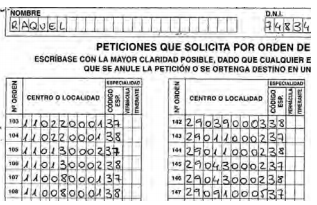
\includegraphics[width=250pt]{../informe/imgs/ejemplo2_anteproyecto.png}
\caption[h]{Ejemplo de formulario}
\end{center}
\end{figure}

\end{itemize}

\section{Dificultades encontradas por el reconocimiento óptico de caracteres}

Existen varias dificultades a la hora de reconocer caracteres. Entre ellas se encuentran:
\begin{itemize}
 \item \textbf{Caligrafía:} Más allá de que los caracteres manuscritos siguen una forma básica, cada persona les aplica ciertos rasgos personales que los hacen únicos. Por ejemplo, un mismo caracter puede tener distinta firmeza en el trazo, distinta inclinación o distinto tamaño, dificultando su reconocimiento.

\begin{figure}[H] %[h] Aqui [b] para button [t] para top
\begin{center}

\includegraphics[width=200pt]{../informe/imgs/ejemplo1_anteproyecto.png}
\caption[h]{Ejemplo de cinco caracteres iguales pero con distinta caligrafía.}
\end{center}
\end{figure}

\item \textbf{Ruido en la imagen:} Como las imágenes se obtienen a partir de un dispositivo, ya sea escáner o cámara de fotos, éste puede agregarle ruido si es que no es muy preciso, como también disminuir la resolución o calidad de la imagen. Llamamos ruido a la variación del brillo o color en las imágenes, como también a las irregularidades que pueden presentar. De este modo, ciertos dispositivos pueden alterar la escala de grises en el fondo de las mismas o sobre los caracteres que posee dificultando el reconocimiento de los mismos. 
Por otro lado, muchos textos se borronean, manchan o tornan amarillos a medida que pasa el tiempo generando ruido y dificultando enormemente la identificación de sus respectivos caracteres.
\end{itemize}

Las características mencionadas anteriormente dificultan el reconocimiento óptico de caracteres y no permiten que el resultado del mismo sea óptimo en todos los casos.

\section{Nuestro proyecto}
El objetivo del trabajo práctico consiste en implementar un método de reconocimiento de dígitos manuscritos basado en la descomposición en valores singulares. Para ello, se procederá utilizando la herramienta de SIMD vista en la materia. De este modo, dada una imagen presentando un número entre 0 y 9, se tomará la información relevante de la misma que permita reconocer digitalmente de qué dígito se trata. El prodecimiento a realizar es el siguiente:
Como instancias de entrenamiento, se tiene un conjunto de $n$ imágenes de dígitos manuscritos en escala de grises del mismo tamaño y resolución (varias imágenes de cada dígito). Cada una de estas imágenes sabemos a que dígito se corresponde pues se encuentran etiquetadas. En este trabajo consideraremos la base de datos MNIST\footnote{http://yann.lecun.com/exdb/mnist/}, utilizada como referencia en esta área de investigación. Para i = 1,..,$n$, sea $x_{i} \in R^{m}$ la i-$ésima$ imagen de nuestra base de datos almacenada por filas en un vector, y sea $\mu$ = ($x_{1}$+...+ $x_{n}$)=$n$ el promedio de las imágenes. Definimos $X \in R_{nxm}$ como la matriz que contiene en la i-$ésima$ fila al vector ($x_{i} - \mu)^t \div \sqrt{n-1}$ y $$X = U \Sigma V^t$$
a su descomposición en valores singulares, con $U \in R^{nxn}$ y $V \in R^{mxm}$ matrices ortogonales, y $\Sigma \in R^{nxm}$ la matriz diagonal conteniendo en la posición $(i, i)$ al i-$ésimo$ valor singular $\sigma_i$.
Siendo $v_i$ la columna $i$ de V, definimos para $i = 1,..,n$ la transformación característica del dígito $x_i$ como el vector $tc(x_i)$ = ($v_1^t
x_i, v_2^t x_i,..., v_k^t x_i) \in R^k$, donde $k \in f_1$,...,m es un parámetro de la implementación. Este proceso corresponde a extraer las $k$ primeras componentes principales de cada imagen. La intención es que $tc(xi)$ resuma la información más relevante de la imagen, descartando los detalles o las zonas que no aportan rasgos distintivos.

Luego, dada una nueva imagen $x$ de un dígito manuscrito, que no se encuentra en el conjunto inicial de imágenes de entrenamiento, el problema de reconocimiento consiste en determinar a qué dígito corresponde. Para esto, se calcula $tc(x)$ y se compara con $tc(x_i)$, para i = 1,...,$n$.

Este proyecto nos pareció oportuno como trabajo final ya que para poder realizarlo es necesario utilizar operaciones sobre matrices. Algunas de estas operaciones, como la triangulación de matrices o la obtención de autovalores y autovectores, pueden ser optimizadas mediante SSE. Esto se debe a que aplican las mismas operaciones sencillas sobre un grupo de elementos, luego, las imágenes podrán ser procesadas a gran velocidad.

Nuestra propuesta consiste en programar tanto en $C$ como en $Assembler$ las funciones principales de los algoritmos que calculan la información más relevante de cada imagen. Una vez hecho esto, analizaremos los tiempos de corrida y evaluaremos la optimización de los mismos.

\section{Tecnologías a utilizar}

Para la realización del trabajo descrito anteriormente, utilizaremos la base de datos MNIST que se encuentra compuesta por imágenes en escala de grises de tamaño 28x28, y presenta un conjunto de entrenamiento de 60000 patrones y uno de testeo de 10000. Aunque ambas bases de datos incluyen casos de dígitos con distorsiones y ambigüedades y que son difíciles de clasificar, la base de datos MNIST tiene en su tratamiento la dificultad de el gran volumen de datos a procesar.

\section{Referencias}
\begin{itemize}
\item http://www.iti.es/media/about/docs/tic/13/articulo2.pdf
\end{itemize}

\end{document}